\documentclass[a4paper, 11pt]{article}
\usepackage[utf8]{inputenc}
\usepackage[english,russian]{babel}
\usepackage[T1, T2A]{fontenc}
\usepackage{graphicx}

\usepackage{pgfplots}
\usetikzlibrary{pgfplots.polar}
\pgfplotsset{compat=1.13, grid=major}
\usepackage[left = 2cm, right = 2cm, bottom = 2cm, top = 2cm]{geometry}
\usepackage[top=2cm, left=2cm, right=2cm, left=2cm]{geometry}
\usepackage{amsmath}

\usepackage{tabu}
\usepackage{threeparttablex} 
\usepackage{booktabs} 
\usepackage[tableposition=top]{caption}
\usepackage{makecell}

\usepackage{subcaption}
\DeclareCaptionLabelFormat{gostfigure}{Рисунок #2}
\DeclareCaptionLabelFormat{gosttable}{Таблица #2}
\DeclareCaptionLabelSeparator{gost}{~---~}
\captionsetup{labelsep=gost}
\captionsetup[figure]{labelformat=gostfigure}
\captionsetup[table]{labelformat=gosttable}
\renewcommand{\thesubfigure}{\asbuk{subfigure}}
\captionsetup[table]{labelformat=simple, labelsep = endash, justification = raggedright, singlelinecheck = off}
\usepackage{indentfirst}
\graphicspath{{image/}}
\newcommand\tline[2]{$\underset{\text{#1}}{\text{\underline{\hspace{#2}}}}$}

% PGFPlots Table ========================================================
\usepackage{pgfplotstable}
\renewcommand{\arraystretch}{1.5}
% pgfplotstable settings
\pgfplotstableset{
    columns/w/.style = {column name = {\boldmath$\omega$}, column type = |c},
    columns/lg_w/.style = {column name = {\boldmath$\lg{\omega}$}, column type = |c},
    columns/A/.style = {column name = {\boldmath$A(\omega)$}, column type = |c},
    columns/L/.style = {column name = {\boldmath$20\lg{A(\omega)}$}, column type = |c},
    columns/psi/.style = {column name = {\boldmath$\psi$}, column type = |c|},
    every head row/.style = {before row = \hline},
    after row = {[1mm] \hline},
}

\begin{document}
	\begin{titlepage}
		\centering
		{\fontsize{12pt}{5cm}\selectfont \bfseries Министерство образования и науки Российской Федерации} \\ \vspace{0.5cm}
		{\fontsize{7pt}{5cm}\selectfont ФЕДЕРАЛЬНОЕ ГОСУДАРСТВЕННОЕ АВТОНОМНОЕ ОБРАЗОВАТЕЛЬНОЕ УЧРЕЖДЕНИЕ ВЫСШЕГО ПРОФЕССИОНАЛЬНОГО ОБРАЗОВАНИЯ} \\ 
		\vspace{1cm}
		{\fontsize{12pt}{5cm}\selectfont \bfseries САНКТ-ПЕТЕРБУРГСКИЙ УНИВЕРСИТЕТ ИНФОРМАЦИОННЫХ ТЕХНОЛОГИЙ, МЕХАНИКИ И ОПТИКИ} \\ \vspace{1.5cm}

		{\fontsize{14pt}{5cm}\selectfont Кафедра \hspace{1cm} \underline{Систем Управления и Информатики}  \hspace{1cm} Группа \underline{Р3340}} \\ 
		\vspace{2cm}

		{\fontsize{20pt}{5cm}\selectfont \bfseries Лабораторная работа №10} \\
		{\fontsize{20pt}{5cm}\selectfont \bfseries “Исследование математической модели электромеханического объекта управления	”} \\
		{\fontsize{14pt}{5cm}\selectfont Вариант - 7} \\
		\vspace{1.5cm}

		\flushleft

		{Выполнил \hspace{2cm} \tline{(фамилия, и.о.)}{9cm} (подпись)} \\
		\vspace{2cm}

		{Проверил \hspace{2cm} \tline{(фамилия, и.о.)}{9cm} (подпись)} \\
		\vspace{5cm}

		"\underline{\hspace{0.7cm}}"\hspace{0.2cm}\underline{\hspace{2cm}}\hspace{0.2cm}20\underline{\hspace{0.7cm}}г. \hspace{2cm} Санкт-Петербург, \hspace{2cm} 20\underline{\hspace{0.7cm}}г. \\ \vspace{1cm}

		Работа выполнена с оценкой \hspace{1cm} \underline{\hspace{8cm}} \\ 
		\vspace{1cm}
		Дата защиты "\underline{\hspace{0.7cm}}"\hspace{0.2cm}\underline{\hspace{2cm}}\hspace{0.2cm}20\underline{\hspace{0.7cm}}г.

\end{titlepage}

\begin{center}
	\section{Задание}
\end{center}
\subsection*{Цель работы} 
\par
Изучение математических моделей и исследование характеристик электромеханического объекта управления(ЭМО), построенного на основе электродвигателя постоянного тока независимого возбуждения.
\par 
В работе исследуется полная и упрощённая модели ЭМО. На рисунке 1 представлена функциональная схема исследуемого объекта.

\begin{figure}[h]
	\center{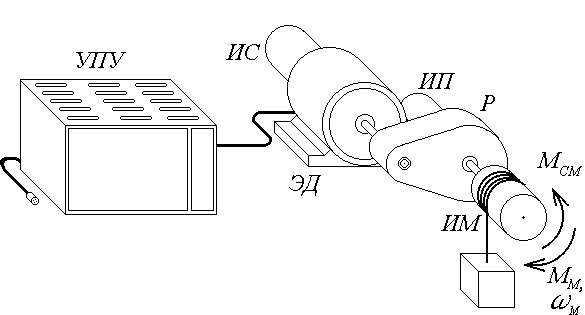
\includegraphics[width=0.75\linewidth]{image/EMO.png}}
	\caption{Функциональная схема исследуемого объекта}
	\label{ris:image}
\end{figure}

\subsection*{Исходные данные}
Исходные данные для моделирования преставлены в таблице 1.

\begin{table}[h!]
	\centering
	\begin{threeparttable}
    	\caption{Исходные данные}\label{tab:perflogcross}
    	\begin{tabular}{|c|c|c|c|c|c|c|c|c|c|}
    		\hline
    		\makecell{$U_\text{Н},$\\В} & \makecell{$n_0,$\\об/мин} & \makecell{$I_\text{Н},$\\A} & \makecell{$M_\text{Н},$\\Н$\cdot$м} & \makecell{R,\\Ом} & \makecell{$T_\text{я},$\\мс} & \makecell{$J_\text{д},$\\кг$\cdot$м$^2$} & \makecell{$T_\text{У},$\\мс} & $i_\text{Р}$ & \makecell{$J_\text{М},$\\кг$\cdot$м$^2$} \\
    		\hline
    		52 & 1240 & 18 & 7.21 & 0.3 & $10\cdot10^-3$ &  0.004 & $10\cdot10^-3$ & 20 & 2.48\\
    		\hline
    	\end{tabular}
    \end{threeparttable}
\end{table}

\newpage
\begin{center}
	\section{Расчёт параметров математического моделирования}
\end{center}
\begin{align*} 
	\displaystyle k_\text{д}=\frac{1}{R}
\end{align*}
\begin{align*}
	\displaystyle k_y = \frac{U_\text{Н}}{U_m}=\frac{52}{10}=5.2
\end{align*}
\begin{align*}
	\displaystyle k_\text{М} = \frac{M_\text{Н}}{I_\text{Н}}=\frac{7.21}{18}=0.4
\end{align*}
\begin{align*}
	\displaystyle k_e = \frac{U_\text{Н}}{\omega_0}=\frac{52\cdot30}{1240\cdot\pi}=0.4
\end{align*}
\begin{align*}
	\displaystyle J_\Sigma=1.2J_\text{д}+\frac{J_M}{i_p^2}=1.2\cdot0.004+\frac{2.48}{20^2}=0.011
\end{align*}

\par 
Коэффициенты передачи измерительных устройств выбираются таким образом, чтобы обеспечить соответствие максимального значения измеряемого сигнала уровню $10 В$ на выходе измерительного устройства.

\begin{align*}
	\displaystyle K_U = 0.1923
\end{align*}
\begin{align*}
	\displaystyle K_I = 0.1082
\end{align*}
\begin{align*}
	\displaystyle K_\omega = 0.0770
\end{align*}
\begin{align*}
	\displaystyle K_\alpha = 1.5888
\end{align*}

\newpage 
\begin{center}
	\section{Вывод математических моделей вход-состояние-выход для полной и упрощенной схем моделирования ЭМО}
\end{center}
\par 
Выведем математическую модель ВСВ для полной схемы моделирования ЭМО. Запишем уравнения, описывающие работу ЭМО:
\begin{equation}
	\displaystyle \begin{cases}
		\displaystyle k_MI-M_c = J_\Sigma\frac{d\omega}{dt}\\
		\displaystyle T_\text{я}\frac{dI}{dt}+I = k_\text{д}(U_y-k_e\omega)\\
		\displaystyle T_y\frac{dU_y}{dt}+U_y = k_yU\\
	\end{cases}
	\Rightarrow
	\begin{cases}
		\displaystyle \dot{\omega} = \displaystyle\frac{k_MI-M_c}{J_\Sigma}\\
		\displaystyle \dot{I} = \displaystyle \frac{k_\text{д}(U_y-k_e\omega)-I}{T_\text{я}}\\
		\displaystyle \dot{U_y} = \displaystyle \frac{k_yU-U_y}{T_y}\\
	\end{cases}
\end{equation}
\par 
Пусть $X = \begin{bmatrix}
	\alpha & \omega & I & U_y
\end{bmatrix}^T$ - вектор состояния, а $U = \begin{bmatrix}
	U & M_c
\end{bmatrix}^T$ - вектор входных воздействий. Тогда 
\begin{equation}
	\begin{cases}
		\dot{X} = AX+BU\\
		y = CX
	\end{cases}
\end{equation}
\begin{align}
	\dot{\alpha} = \omega
\end{align}

\begin{equation}
	\begin{bmatrix}
		\dot{\alpha}\\
		\dot{\omega}\\
		\dot{I}\\
		\dot{U_y}\\
	\end{bmatrix}
	=
	\begin{bmatrix}
		\displaystyle 0 & 1 & 0 & 0 \\
		\displaystyle 0 & 0 & \displaystyle\frac{k_M}{J_\Sigma} & 0 \\
		\displaystyle 0 & \displaystyle -\frac{k_ek_\text{д}}{T_\text{я}} & \displaystyle -\frac{1}{T_\text{я}} & \displaystyle \frac{k_\text{д}}{T_\text{я}} \\
		\displaystyle 0 & 0 & 0 & \displaystyle -\frac{1}{T_y}\\
	\end{bmatrix}
	\cdot 
	\begin{bmatrix}
		{\alpha}\\
		{\omega}\\
		{I}\\
		{U_y}\\
	\end{bmatrix}
	+
	\begin{bmatrix}
		0 & 0 \\
		\displaystyle 0 & \displaystyle -\frac{1}{J_\Sigma} \\
		0 & 0 \\
		\displaystyle \frac{k_y}{T_y} & 0 \\
	\end{bmatrix}
	\cdot
	\begin{bmatrix}
		U\\
		M_c\\
	\end{bmatrix}
\end{equation}
\par 
Запишем матрицы A, B и C:
\begin{equation}
	A = 
	\begin{bmatrix}
		\displaystyle 0 & 1 & 0 & 0\\
		\displaystyle 0 & 0 & \frac{k_M}{J_\Sigma} & 0\\
		\displaystyle 0 & \displaystyle -\frac{k_ek_\text{д}}{T_\text{я}} & \displaystyle -\frac{1}{T_\text{я}} & \displaystyle \frac{k_\text{д}}{T_\text{я}}\\
		\displaystyle 0 & 0 & 0 & \displaystyle -\frac{1}{T_\text{я}}\\
	\end{bmatrix}
	,\ B = 
	\begin{bmatrix}
		0 & 0\\
		\displaystyle 0 & \displaystyle -\frac{1}{J_\Sigma}\\
		0 & 0\\
		\displaystyle \frac{k_y}{T_y} & 0\\
	\end{bmatrix}
	, \ C = 
	\begin{bmatrix}
		1 & 0 & 0 & 0\\
	\end{bmatrix}
\end{equation}

\par 
Выведем математическую модель упрощенной схемы моделирования ЭМО. Она получается в результате пренебрежения малыми постоянными времени $T_\text{я}$ и $T_y$.
\begin{equation}
	\begin{cases}
		\dot{\alpha} = \omega\\
		\displaystyle \dot{\omega} = -\frac{k_Mk_\text{д}k_e}{J_\Sigma} \omega+\frac{k_Mk_\text{д}k_y}{J_\Sigma} U-\frac{1}{J_\Sigma}M_c\\
	\end{cases}
\end{equation}
\par
Таким образом, получаем модель ВСВ:
\begin{equation}
	\begin{bmatrix}
		\dot{\alpha}\\
		\dot{\omega}\\
	\end{bmatrix}
	=
	\begin{bmatrix}
		0 & 1\\
		\displaystyle 0 & -\frac{k_Mk_\text{Д}k_e}{J_\Sigma}\\
	\end{bmatrix}
	\cdot
	\begin{bmatrix}
		\alpha\\
		\omega\\
	\end{bmatrix}
	+
	\begin{bmatrix}
		0 & 0\\
		\displaystyle \frac{k_Mk_\text{Д}k_y}{J_\Sigma} & -\frac{1}{J_\Sigma}\\
	\end{bmatrix}
	\cdot
	\begin{bmatrix}
		U\\
		M_c\\
	\end{bmatrix}
\end{equation}

\newpage
\begin{center}
	\section{Исследование полной модели ЭМО}
\end{center}
\par 
На рисунке 2 представлена схема полной модели ЭМО.

\begin{figure}[h]
	\center{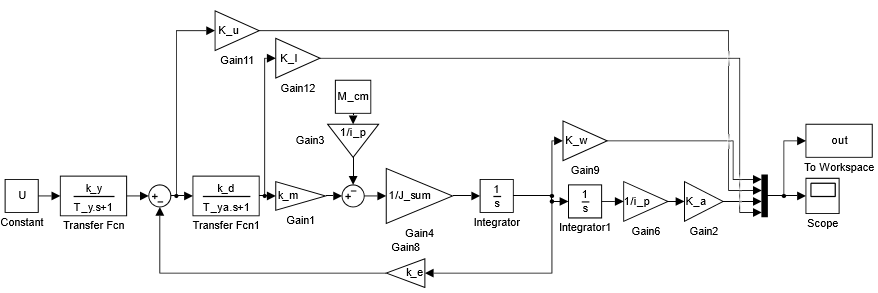
\includegraphics[width=0.95\linewidth]{image/full.png}}
	\caption{Схема полной модели ЭМО}
	\label{ris:image}
\end{figure}
\par 
На рисунке 3 представлены сравнительные графики при различных $T_y$ и $T_\text{я}$. Так как в данном случае $T_y=T_\text{я}$, обозначим $T = T_y = T_\text{я}$.

\newpage
\begin{figure}[h!]
	\begin{subfigure}{0.5\textwidth}
	\centering
		\begin{tikzpicture}
			\begin{axis}[
				xlabel = {\Large{$t,c$}},
				ylabel = {\Large{$U,B$}},
				width = 250,
				height = 220,
				grid = both,
				legend pos = south east,
				extra y ticks = {5},
				legend style={nodes={scale=0.9, transform shape}}
				%extra y tick style={grid style={black, line width = 1}},
				%ytick = {0, 0.2, 0.4, 0.6, 1, 1.2}				
			]

			\addplot[line width = 1] table [x=t, y=U] 
              	{data/2_1.txt};
			\addplot[line width = 1, dotted, draw = blue] table [x=t, y=U]
				{data/2_2.txt};			
			\legend{
				$T = 10\cdot10^{-3}c$,
				$T = 10\cdot10^{-4}c$	
				}
			\end{axis}
		\end{tikzpicture}
		\caption{Результаты моделирования $U$}
    \end{subfigure}
    \begin{subfigure}{0.5\textwidth}
	\centering
		\begin{tikzpicture}
			\begin{axis}[
				xlabel = {\Large{$t,c$}},
				ylabel = {\Large{$I,A$}},
				width = 250,
				height = 220,
				grid = both,
				legend style={nodes={scale=0.9, transform shape}}
			]

			\addplot[line width = 1] table [x=t, y=I] 
              	{data/2_1.txt};
			\addplot[line width = 1, dotted, draw = blue] table [x=t, y=I]
				{data/2_2.txt};			
			\legend{
				$T = 10\cdot10^{-3}c$,
				$T = 10\cdot10^{-4}c$
				}
			\end{axis}
		\end{tikzpicture}
		\caption{Результаты моделирования $I$}
    \end{subfigure}
    
    \vspace{0.5cm}

    \begin{subfigure}{0.5\textwidth}
	\centering
		\begin{tikzpicture}
			\begin{axis}[
				xlabel = {\Large{$t,c$}},
				ylabel = {\Large{$\alpha,\text{рад}$}},
				width = 250,
				height = 220,
				grid = both,
				legend pos = north west,
				legend style={nodes={scale=0.9, transform shape}}
			]

			\addplot[line width = 1] table [x=t, y=a] 
              	{data/2_1.txt};
			\addplot[line width = 1, dotted, draw = blue] table [x=t, y=a]
				{data/2_2.txt};			
			\legend{
				$T = 10\cdot10^{-3}c$,
				$T = 10\cdot10^{-4}c$	
				}
			\end{axis}
		\end{tikzpicture}
		\caption{Результаты моделирования $\alpha$}
    \end{subfigure}
    \begin{subfigure}{0.5\textwidth}
	\centering
		\begin{tikzpicture}
			\begin{axis}[
				xlabel = {\Large{$t,c$}},
				ylabel = {\Large{$\omega,\text{рад/с}$}},
				width = 250,
				height = 220,
				grid = both,
				legend pos = south east,
				extra y ticks = {5},
				legend style={nodes={scale=0.9, transform shape}}
			]
			\addplot[line width = 1] table [x=t, y=w] 
              	{data/2_1.txt};
			\addplot[line width = 1, dotted, draw = blue] table [x=t, y=w]
				{data/2_2.txt};			
			\legend{
				$T = 10\cdot10^{-3}c$,
				$T = 10\cdot10^{-4}c$
				}
			\end{axis}
		\end{tikzpicture}
		\caption{Результаты моделирования $\omega$}
    \end{subfigure}
    \caption{Передаточные характеристики при различных $T_y$ и $T_\text{я}$}
\end{figure}

\par 
Результаты переходных процессов для $T = 10\cdot10^{-3}$:
\begin{equation*}
	t_\text{п} = 0.046,\ \omega_y = 5,\ I = 0
\end{equation*}
\par 
Результаты переходных процессов для $T = 10\cdot10^{-4}$:
\begin{equation*}
	t_\text{п} = 4.285\cdot10^-{3},\ \omega_y = 5,\ I = 0
\end{equation*}

\newpage
\begin{center}
	\section{Исследование влияния нагрузочного момента}
\end{center}
\par 
На рисунке 4 представлены сравнительные графики при различных значениях нагрузочного момента.

\begin{figure}[h!]
	\begin{subfigure}{0.5\textwidth}
	\centering
		\begin{tikzpicture}
			\begin{axis}[
				%scale only axis,
				xlabel = {\Large{$t,c$}},
				ylabel = {\Large{$U,B$}},
				width = 250,
				height = 220,
				grid = both,
				legend pos = south east,
				extra y ticks = {5},
				legend style={nodes={scale=0.9, transform shape}}
			]
			\addplot[line width = 1, draw = blue] table [x=t, y=M_28]
				{data/3_u.txt};
			\end{axis}
		\end{tikzpicture}
		\caption{Результаты моделирования $U$}
    \end{subfigure}
    \begin{subfigure}{0.5\textwidth}
	\centering
		\begin{tikzpicture}
			\begin{axis}[
				xlabel = {\Large{$t,c$}},
				ylabel = {\Large{$I,A$}},
				width = 250,
				height = 220,
				grid = both,
				extra y ticks = {0.39, 0.78, 1.17, 1.56, 1.95},
				ytick = {0, 4, 6},
				%scale only axis,
				enlarge y limits=0.05,
				legend style={nodes={scale=0.9, transform shape}}
			]

			\addplot[line width = 1, densely dashdotted, draw = blue] table [x=t, y=M_28]
				{data/3_i.txt};
			\addplot[line width = 1, densely dashed, draw = purple] table [x=t, y=M_57]
				{data/3_i.txt};
			\addplot[line width = 1, dashdotted, draw = gray] table [x=t, y=M_86]
				{data/3_i.txt};
			\addplot[line width = 1, loosely dotted, draw = red] table [x=t, y=M_115]
				{data/3_i.txt};	
			\addplot[line width = 1] table [x=t, y=M_144] 
              	{data/3_i.txt};			
			\legend{
				$M = 28\ H\text{м}$,
				$M = 57\ H\text{м}$,
				$M = 86\ H\text{м}$,
				$M = 115\ H\text{м}$,
				$M = 144\ H\text{м}$	
				}
			\end{axis}
		\end{tikzpicture}
		\caption{Результаты моделирования $I$}
    \end{subfigure}
    
    \vspace{0.5cm}

    \begin{subfigure}{0.5\textwidth}
	\centering
		\begin{tikzpicture}
			\begin{axis}[
				%scale only axis,
				xlabel = {\Large{$t,c$}},
				ylabel = {\Large{$\alpha,\text{рад}$}},
				width = 250,
				height = 220,
				grid = both,
				legend pos = north west,
				legend style={nodes={scale=0.9, transform shape}}
			]

			\addplot[line width = 1, densely dashdotted, draw = blue] table [x=t, y=M_28]
				{data/3_a.txt};
			\addplot[line width = 1, densely dashed, draw = purple] table [x=t, y=M_57]
				{data/3_a.txt};
			\addplot[line width = 1, dashdotted, draw = gray] table [x=t, y=M_86]
				{data/3_a.txt};
			\addplot[line width = 1, loosely dotted, draw = red] table [x=t, y=M_115]
				{data/3_a.txt};	
			\addplot[line width = 1] table [x=t, y=M_144] 
              	{data/3_a.txt};			
			\legend{
				$M = 28\ H\text{м}$,
				$M = 57\ H\text{м}$,
				$M = 86\ H\text{м}$,
				$M = 115\ H\text{м}$,
				$M = 144\ H\text{м}$	
				}
			\end{axis}
		\end{tikzpicture}
		\caption{Результаты моделирования $\alpha$}
    \end{subfigure}
    \begin{subfigure}{0.5\textwidth}
	\centering
		\begin{tikzpicture}
			\begin{axis}[
				%scale only axis,
				samples=60,
    			domain=0:5.05,
    			%y = 2cm, 
    			%restrict y to domain=0:5,
				xlabel = {\Large{$t,c$}},
				ylabel = {\Large{$\omega,\text{рад/с}$}},
				width = 250,
				height = 220,
				grid = both,
				legend pos = south east,
				extra y tick style={y tick label style={font=\tiny,fill=none}},
				extra y ticks = {5, 4.79,4.58,	4.377, 4.17, 3.96},
				enlarge y limits = 0.05,
				legend style={nodes={scale=0.9, transform shape}},
				%ticklabel style={font=\large,fill=none},
				ytick = {0,1,2,3},
				xtick = {0,0.05, 0.1, 0.15, 0.2, 0.25, 0.3}
			]

			\addplot[line width = 1, densely dashdotted, draw = blue] table [x=t, y=M_28]
				{data/3_w.txt};
			\addplot[line width = 1, densely dashed, draw = purple] table [x=t, y=M_57]
				{data/3_w.txt};
			\addplot[line width = 1, dashdotted, draw = gray] table [x=t, y=M_86]
				{data/3_w.txt};
			\addplot[line width = 1, loosely dotted, draw = red] table [x=t, y=M_115]
				{data/3_w.txt};	
			\addplot[line width = 1] table [x=t, y=M_144] 
              	{data/3_w.txt};				
			\legend{
				$M = 28\ H\text{м}$,
				$M = 57\ H\text{м}$,
				$M = 86\ H\text{м}$,
				$M = 115\ H\text{м}$,
				$M = 144\ H\text{м}$
				}
			\end{axis}
		\end{tikzpicture}
		\caption{Результаты моделирования $\omega$}
    \end{subfigure}
    \caption{Характеристики при различных нагрузочных моментах}
\end{figure}

\par 
В таблице 2 представлены результаты моделирования при различных нагрузочных моментах.
\newpage
\begin{table}[h!]
\centering
	\begin{threeparttable}
	\caption{Результаты моделирования}\label{tab:perflogcross}
		\begin{tabular}{|c|c|c|c|}
			\hline
			$M$ & $t_\text{п}$ & $\omega$ & I\\
			\hline
			28 & 0.0461 & 4.79 & 0.39\\
			\hline
			57 & 0.0461 & 4.58 & 0.78\\
			\hline
			86 & 0.0461 & 4.38 & 1.17\\
			\hline
			115 & 0.0561 & 4.17 & 1.56\\
			\hline
			144 & 0.0461 & 3.96 & 1.95\\
			\hline
		\end{tabular}
	\end{threeparttable}
\end{table}

\newpage
\begin{center}
	\section{Исследование влияния момента инерции}
\end{center}
\par 
На рисунке 5 представлены результаты моделирования при различных моментах инерции $J_m$.

\begin{figure}[h!]
	\begin{subfigure}{0.5\textwidth}
	\centering
		\begin{tikzpicture}
			\begin{axis}[
				xlabel = {\Large{$t,c$}},
				ylabel = {\Large{$U,B$}},
				width = 250,
				height = 220,
				grid = both,
				legend pos = south east,
				legend style={nodes={scale=0.9, transform shape}}
			]
			\addplot[line width = 1, densely dashdotted, draw = blue] table [x=t, y=J_124]
				{data/4_u.txt};			
			\end{axis}
		\end{tikzpicture}
		\caption{Результаты моделирования $U$}
    \end{subfigure}
    \begin{subfigure}{0.5\textwidth}
	\centering
		\begin{tikzpicture}
			\begin{axis}[
				xlabel = {\Large{$t,c$}},
				ylabel = {\Large{$I,A$}},
				width = 250,
				height = 220,
				grid = both,
				legend style={nodes={scale=0.9, transform shape}}
			]

			\addplot[line width = 1, densely dashdotted, draw = blue] table [x=t, y=J_124]
				{data/4_i.txt};
			\addplot[line width = 1, densely dashed, draw = purple] table [x=t, y=J_186]
				{data/4_i.txt};
			\addplot[line width = 1, dashdotted, draw = gray] table [x=t, y=J_248]
				{data/4_i.txt};
			\addplot[line width = 1, loosely dotted, draw = red] table [x=t, y=J_31]
				{data/4_i.txt};	
			\addplot[line width = 1] table [x=t, y=J_372] 
              	{data/4_i.txt};				
			\legend{
				$J_m = 1.24\ \text{кг}\cdot\text{м}^2$,
				$J_m = 1.86\ \text{кг}\cdot\text{м}^2$,
				$J_m = 2.48\ \text{кг}\cdot\text{м}^2$,
				$J_m = 3.1\ \text{кг}\cdot\text{м}^2$,
				$J_m = 3.72\ \text{кг}\cdot\text{м}^2$	
				}
			\end{axis}
		\end{tikzpicture}
		\caption{Результаты моделирования $I$}
    \end{subfigure}
    
    \vspace{0.5cm}

    \begin{subfigure}{0.5\textwidth}
	\centering
		\begin{tikzpicture}
			\begin{axis}[
				xlabel = {\Large{$t,c$}},
				ylabel = {\Large{$\alpha,\text{рад}$}},
				width = 250,
				height = 220,
				grid = both,
				legend pos = north west,
				legend style={nodes={scale=0.9, transform shape}}
			]

			\addplot[line width = 1, densely dashdotted, draw = blue] table [x=t, y=J_124]
				{data/4_a.txt};
			\addplot[line width = 1, densely dashed, draw = purple] table [x=t, y=J_186]
				{data/4_a.txt};
			\addplot[line width = 1, dashdotted, draw = gray] table [x=t, y=J_248]
				{data/4_a.txt};
			\addplot[line width = 1, loosely dotted, draw = red] table [x=t, y=J_31]
				{data/4_a.txt};	
			\addplot[line width = 1] table [x=t, y=J_372] 
              	{data/4_a.txt};				
			\legend{
				$J_m = 1.24\ \text{кг}\cdot\text{м}^2$,
				$J_m = 1.86\ \text{кг}\cdot\text{м}^2$,
				$J_m = 2.48\ \text{кг}\cdot\text{м}^2$,
				$J_m = 3.1\ \text{кг}\cdot\text{м}^2$,
				$J_m = 3.72\ \text{кг}\cdot\text{м}^2$	
				}
				
			\end{axis}
		\end{tikzpicture}
		\caption{Результаты моделирования $\alpha$}
    \end{subfigure}
    \begin{subfigure}{0.5\textwidth}
	\centering
		\begin{tikzpicture}
			\begin{axis}[
				xlabel = {\Large{$t,c$}},
				ylabel = {\Large{$\omega,\text{рад/с}$}},
				width = 250,
				height = 220,
				grid = both,
				legend pos = south east,
				extra y ticks = {5},
				legend style={nodes={scale=0.9, transform shape}}
			]

			\addplot[line width = 1, densely dashdotted, draw = blue] table [x=t, y=J_124]
				{data/4_w.txt};
			\addplot[line width = 1, densely dashed, draw = purple] table [x=t, y=J_186]
				{data/4_w.txt};
			\addplot[line width = 1, dashdotted, draw = gray] table [x=t, y=J_248]
				{data/4_w.txt};
			\addplot[line width = 1, loosely dotted, draw = red] table [x=t, y=J_31]
				{data/4_w.txt};	
			\addplot[line width = 1] table [x=t, y=J_372] 
              	{data/4_w.txt};				
			\legend{
				$J_m = 1.24\ \text{кг}\cdot\text{м}^2$,
				$J_m = 1.86\ \text{кг}\cdot\text{м}^2$,
				$J_m = 2.48\ \text{кг}\cdot\text{м}^2$,
				$J_m = 3.1\ \text{кг}\cdot\text{м}^2$,
				$J_m = 3.72\ \text{кг}\cdot\text{м}^2$	
				}
			\end{axis}
		\end{tikzpicture}
		\caption{Результаты моделирования $\omega$}
    \end{subfigure}
    \caption{Характеристики при различных моментах инерции}
\end{figure}

\par 
В таблице 3 представлены результаты моделирования при различных моментах инерции.
\newpage
\begin{table}[h!]
\centering
	\begin{threeparttable}
	\caption{Результаты моделирования}\label{tab:perflogcross}
		\begin{tabular}{|c|c|c|c|}
			\hline
			$J_m$ & $t_\text{п}$ & $\omega$ & I\\
			\hline
			1.24 & 0.0461 & 5 & 0\\
			\hline
			1.86 & 0.0461 & 5 & 0\\
			\hline
			2.48 & 0.0461 & 5 & 0\\
			\hline
			3.1 & 0.0561 & 5 & 0\\
			\hline
			3.72 & 0.0461 & 5 & 0\\
			\hline
		\end{tabular}
	\end{threeparttable}
\end{table}

\newpage
\begin{center}
	\section{Исследование влияния передаточного отношения}
\end{center}
\par
На рисунке 6 представлены результаты моделирования при $M_{cm} = 0$ и различных передаточных отношениях.

\begin{figure}[h!]
	\begin{subfigure}{0.5\textwidth}
	\centering
		\begin{tikzpicture}
			\begin{axis}[
				xlabel = {\Large{$t,c$}},
				ylabel = {\Large{$U,B$}},
				width = 250,
				height = 220,
				grid = both,
				legend pos = south east,
				legend style={nodes={scale=0.9, transform shape}}
			]
			\addplot[line width = 1, draw = blue] table [x=t, y=i_5]
				{data/5_u_0.txt};
			\end{axis}
		\end{tikzpicture}
		\caption{Результаты моделирования $U$}
    \end{subfigure}
    \begin{subfigure}{0.5\textwidth}
	\centering
		\begin{tikzpicture}
			\begin{axis}[
				xlabel = {\Large{$t,c$}},
				ylabel = {\Large{$I,A$}},
				width = 250,
				height = 220,
				grid = both,
				legend style={nodes={scale=0.9, transform shape}}
			]
			\addplot[line width = 1, dashed, draw = blue] table [x=t, y=i_5]
				{data/5_i_0.txt};
			\addplot[line width = 1, dotted, draw = green] table [x=t, y=i_10]
				{data/5_i_0.txt};
			\addplot[line width = 1, densely dashdotted, draw = yellow] table [x=t, y=i_15]
				{data/5_i_0.txt};
			\addplot[line width = 1, densely dashed, draw = purple] table [x=t, y=i_20]
				{data/5_i_0.txt};
			\addplot[line width = 1, dashdotted, draw = gray] table [x=t, y=i_25]
				{data/5_i_0.txt};
			\addplot[line width = 1, loosely dotted, draw = red] table [x=t, y=i_30]
				{data/5_i_0.txt};	
			\addplot[line width = 1] table [x=t, y=i_35] 
              	{data/5_i_0.txt};		
			\legend{
				$i_p = 5$,
				$i_p = 10$,
				$i_p = 15$,
				$i_p = 20$,
				$i_p = 25$,
				$i_p = 30$,
				$i_p = 35$
				}
			\end{axis}
		\end{tikzpicture}
		\caption{Результаты моделирования $I$}
    \end{subfigure}    
    \vspace{0.5cm}
    \begin{subfigure}{0.5\textwidth}
	\centering
		\begin{tikzpicture}
			\begin{axis}[
				xlabel = {\Large{$t,c$}},
				ylabel = {\Large{$\alpha,\text{рад}$}},
				width = 250,
				height = 220,
				grid = both,
				legend pos = north west,
				legend style={nodes={scale=0.9, transform shape}}
			]
			\addplot[line width = 1, dashed, draw = blue] table [x=t, y=i_5]
				{data/5_a_0.txt};
			\addplot[line width = 1, dotted, draw = green] table [x=t, y=i_10]
				{data/5_a_0.txt};
			\addplot[line width = 1, densely dashdotted, draw = yellow] table [x=t, y=i_15]
				{data/5_a_0.txt};
			\addplot[line width = 1, densely dashed, draw = purple] table [x=t, y=i_20]
				{data/5_a_0.txt};
			\addplot[line width = 1, dashdotted, draw = gray] table [x=t, y=i_25]
				{data/5_a_0.txt};
			\addplot[line width = 1, loosely dotted, draw = red] table [x=t, y=i_30]
				{data/5_a_0.txt};	
			\addplot[line width = 1] table [x=t, y=i_35] 
              	{data/5_a_0.txt};		
			\legend{
				$i_p = 5$,
				$i_p = 10$,
				$i_p = 15$,
				$i_p = 20$,
				$i_p = 25$,
				$i_p = 30$,
				$i_p = 35$
				}
			\end{axis}
		\end{tikzpicture}
		\caption{Результаты моделирования $\alpha$}
    \end{subfigure}
    \begin{subfigure}{0.5\textwidth}
	\centering
		\begin{tikzpicture}
			\begin{axis}[
				xlabel = {\Large{$t,c$}},
				ylabel = {\Large{$\omega,\text{рад/с}$}},
				width = 250,
				height = 220,
				grid = both,
				legend pos = south east,
				legend style={nodes={scale=0.9, transform shape}},
				extra y ticks = {5}
			]

			\addplot[line width = 1, dashed, draw = blue] table [x=t, y=i_5]
				{data/5_w_0.txt};
			\addplot[line width = 1, dotted, draw = green] table [x=t, y=i_10]
				{data/5_w_0.txt};
			\addplot[line width = 1, densely dashdotted, draw = yellow] table [x=t, y=i_15]
				{data/5_w_0.txt};
			\addplot[line width = 1, densely dashed, draw = purple] table [x=t, y=i_20]
				{data/5_w_0.txt};
			\addplot[line width = 1, dashdotted, draw = gray] table [x=t, y=i_25]
				{data/5_w_0.txt};
			\addplot[line width = 1, loosely dotted, draw = red] table [x=t, y=i_30]
				{data/5_w_0.txt};	
			\addplot[line width = 1] table [x=t, y=i_35] 
              	{data/5_w_0.txt};		
			\legend{
				$i_p = 5$,
				$i_p = 10$,
				$i_p = 15$,
				$i_p = 20$,
				$i_p = 25$,
				$i_p = 30$,
				$i_p = 35$
				}
			\end{axis}
		\end{tikzpicture}
		\caption{Результаты моделирования $\omega$}
    \end{subfigure}
    \caption{Характеристики при различных передаточных отношениях и $M_{cm}=0$}
\end{figure}

\par
В таблице 4 представлены результаты моделирования при различных передаточных отношениях и нулевом нагрузочном моменте.
\newpage
\begin{table}[h!]
\centering
	\begin{threeparttable}
	\caption{Результаты моделирования}\label{tab:perflogcross}
		\begin{tabular}{|c|c|c|c|}
			\hline
			$i_p$ & $t_\text{п}$ & $\omega$ & I\\
			\hline
			1.24 & 0.0461 & 5 & 0\\
			\hline
			1.86 & 0.0461 & 5 & 0\\
			\hline
			2.48 & 0.0461 & 5 & 0\\
			\hline
			3.1 & 0.0561 & 5 & 0\\
			\hline
			3.72 & 0.0461 & 5 & 0\\
			\hline
		\end{tabular}
	\end{threeparttable}
\end{table}

\par
На рисунке 7 представлены результаты моделирования при $M_{cm}=72$ и различных передаточных отношениях. Ввиду нечитаемого расположения подписей, на рисунке 7 представлено меньшее число линий для тока и угловой скорости.
\newpage
\begin{figure}[h!]
	\begin{subfigure}{0.5\textwidth}
	\centering
		\begin{tikzpicture}
			\begin{axis}[
				xlabel = {\Large{$t,c$}},
				ylabel = {\Large{$U,B$}},
				width = 250,
				height = 220,
				grid = both,
				legend pos = south east,
				legend style={nodes={scale=0.9, transform shape}}
			]
			\addplot[line width = 1, draw = blue] table [x=t, y=i_5]
				{data/5_u.txt};		
			\end{axis}
		\end{tikzpicture}
		\caption{Результаты моделирования $U$}
    \end{subfigure}
    \begin{subfigure}{0.5\textwidth}
	\centering
		\begin{tikzpicture}
			\begin{axis}[
				xlabel = {\Large{$t,c$}},
				ylabel = {\Large{$I,A$}},
				width = 250,
				height = 220,
				grid = both,
				legend style={nodes={scale=0.9, transform shape}},
				extra y tick style={y tick label style={font=\large,fill=none}},
				extra y ticks = {3.89, 1.94, 1.297, 0.556},
				ytick = {0,6,8}
			]
			\addplot[line width = 1, dashed, draw = blue] table [x=t, y=i_5]
				{data/5_i.txt};
			\addplot[line width = 1, dotted, draw = green] table [x=t, y=i_10]
				{data/5_i.txt};
			\addplot[line width = 1, densely dashdotted, draw = red] table [x=t, y=i_15]
				{data/5_i.txt};
			%\addplot[line width = 1, densely dashed, draw = purple] table [x=t, y=i_20]
				%{data/5_i.txt};
			%\addplot[line width = 1, dashdotted, draw = gray] table [x=t, y=i_25]
				%{data/5_i.txt};
			%\addplot[line width = 1, loosely dotted, draw = red] table [x=t, y=i_30]
				%{data/5_i.txt};	
			\addplot[line width = 1] table [x=t, y=i_35] 
              	{data/5_i.txt};		
			\legend{
				$i_p = 5$,
				$i_p = 10$,
				$i_p = 15$,
				%$i_p = 20$,
				%$i_p = 25$,
				%$i_p = 30$,
				$i_p = 35$
				}
			\end{axis}
		\end{tikzpicture}
		\caption{Результаты моделирования $I$}
    \end{subfigure}    
    \vspace{0.5cm}
    \begin{subfigure}{0.5\textwidth}
	\centering
		\begin{tikzpicture}
			\begin{axis}[
				xlabel = {\Large{$t,c$}},
				ylabel = {\Large{$\alpha,\text{рад}$}},
				width = 250,
				height = 220,
				grid = both,
				legend pos = north west,
				legend style={nodes={scale=0.9, transform shape}}
			]
			\addplot[line width = 1, dashed, draw = blue] table [x=t, y=i_5]
				{data/5_a.txt};
			\addplot[line width = 1, dotted, draw = green] table [x=t, y=i_10]
				{data/5_a.txt};
			\addplot[line width = 1, densely dashdotted, draw = yellow] table [x=t, y=i_15]
				{data/5_a.txt};
			\addplot[line width = 1, densely dashed, draw = purple] table [x=t, y=i_20]
				{data/5_a.txt};
			\addplot[line width = 1, dashdotted, draw = gray] table [x=t, y=i_25]
				{data/5_a.txt};
			\addplot[line width = 1, loosely dotted, draw = red] table [x=t, y=i_30]
				{data/5_a.txt};	
			\addplot[line width = 1] table [x=t, y=i_35] 
              	{data/5_a.txt};		
			\legend{
				$i_p = 5$,
				$i_p = 10$,
				$i_p = 15$,
				$i_p = 20$,
				$i_p = 25$,
				$i_p = 30$,
				$i_p = 35$
				}
			\end{axis}
		\end{tikzpicture}
		\caption{Результаты моделирования $\alpha$}
    \end{subfigure}
    \begin{subfigure}{0.5\textwidth}
	\centering
		\begin{tikzpicture}
			\begin{axis}[
				xlabel = {\Large{$t,c$}},
				ylabel = {\Large{$\omega,\text{рад/с}$}},
				width = 250,
				height = 220,
				grid = both,
				legend pos = south east,
				legend style={nodes={scale=0.9, transform shape}},
				extra y tick style={y tick label style={font=\large,fill=none}},
				extra y ticks = {2.926, 3.963, 4.31, 4.7},
				ytick = {0,1,2,5},
			]

			\addplot[line width = 1, dashed, draw = blue] table [x=t, y=i_5]
				{data/5_w.txt};
			\addplot[line width = 1, dotted, draw = green] table [x=t, y=i_10]
				{data/5_w.txt};
			\addplot[line width = 1, densely dashdotted, draw = red] table [x=t, y=i_15]
				{data/5_w.txt};
			%\addplot[line width = 1, densely dashed, draw = purple] table [x=t, y=i_20]
				%{data/5_w.txt};
			%\addplot[line width = 1, dashdotted, draw = gray] table [x=t, y=i_25]
				%{data/5_w.txt};
			%\addplot[line width = 1, loosely dotted, draw = red] table [x=t, y=i_30]
				%{data/5_w.txt};	
			\addplot[line width = 1] table [x=t, y=i_35] 
              	{data/5_w.txt};		
			\legend{
				$i_p = 5$,
				$i_p = 10$,
				$i_p = 15$,
				%$i_p = 20$,
				%$i_p = 25$,
				%$i_p = 30$,
				$i_p = 35$
				}
			\end{axis}
		\end{tikzpicture}
		\caption{Результаты моделирования $\omega$}
    \end{subfigure}
    \caption{Характеристики при различных передаточных отношениях и $M_{cm}=72$}
\end{figure}

\par
В таблице 5 представлены результаты моделирования при $M_{cm}=72$ и различных передаточных отношениях.
\begin{table}[h!]
\centering
	\begin{threeparttable}
	\caption{Результаты моделирования}\label{tab:perflogcross}
		\begin{tabular}{|c|c|c|c|}
			\hline
			$i_p$ & $t_\text{п}$ & $\omega$ & I\\
			\hline
			5 & 0.0461 & 2.926 & 3.89\\
			\hline
			10 & 0.0461 & 3.963 & 1.94\\
			\hline
			15 & 0.0461 & 4.31 & 1.297\\
			\hline
			35 & 0.0561 & 4.7 & 0.556\\
			\hline
		\end{tabular}
	\end{threeparttable}
\end{table}

\newpage
\begin{center}
	\section{Исследование упрощённой модели ЭМО и сравнение с полной}
\end{center}
\par 
На рисунке 8 представлена упрощённая схема моделирования ЭМО.

\begin{figure}[h]
	\center{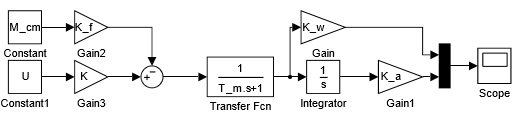
\includegraphics[width=0.75\linewidth]{image/easy.png}}
	\caption{Схема упрощённой модели ЭМО}
	\label{ris:image}
\end{figure}

\par 
На рисунке 9 представлены сравнительные графики для полной и упрощённой моделей ЭМО при различных значениях $T=T_y=T_\text{я}$.

\begin{figure}[h!]
	\begin{subfigure}{0.5\textwidth}
	\centering
		\begin{tikzpicture}
			\begin{axis}[
				xlabel = {\Large{$t,c$}},
				ylabel = {\Large{$\omega,\text{рад/с}$}},
				width = 220,
				height = 200,
				grid = both,
				legend pos = south east,
				extra y ticks = {5}
			]

			\addplot[line width = 1] table [x=t, y=w_full] 
              	{data/6_1.txt};
			\addplot[line width = 1, dotted, draw = blue] table [x=t, y=w_easy]
				{data/6_1.txt};			
			\legend{
				$\omega_{full}$,
				$\omega_{easy}$		
				}
			\end{axis}
		\end{tikzpicture}
		\caption{Результаты моделирования $T = 10\cdot10^{-3}$}
    \end{subfigure}
    \begin{subfigure}{0.5\textwidth}
	\centering
		\begin{tikzpicture}
			\begin{axis}[
				xlabel = {\Large{$t,c$}},
				ylabel = {\Large{$\omega,\text{рад/с}$}},
				width = 220,
				height = 200,
				grid = both,
				legend pos = south east,
			]

			\addplot[line width = 1] table [x=t, y=w_full] 
              	{data/6_2.txt};
			\addplot[line width = 1, dotted, draw = blue] table [x=t, y=w_easy]
				{data/6_2.txt};			
			\legend{
				$\omega_{full}$,
				$\omega_{easy}$	
				}
			\end{axis}
		\end{tikzpicture}
		\caption{Результаты моделирования $T = 10\cdot10^{-4}$}
    \end{subfigure}
    \vspace{0.5cm}
    \begin{subfigure}{0.5\textwidth}
	\centering
		\begin{tikzpicture}
			\begin{axis}[
				xlabel = {\Large{$t,c$}},
				ylabel = {\Large{$\alpha,\text{рад}$}},
				width = 220,
				height = 200,
				grid = both,
				legend pos = north west,
			]

			\addplot[line width = 1] table [x=t, y=a_full] 
              	{data/6_1.txt};
			\addplot[line width = 1, dotted, draw = blue] table [x=t, y=a_easy]
				{data/6_1.txt};			
			\legend{
				$\alpha_{full}$,
				$\alpha_{easy}$	
				}
			\end{axis}
		\end{tikzpicture}
		\caption{Результаты моделирования $T = 10\cdot10^{-3}$}
    \end{subfigure}
    \begin{subfigure}{0.5\textwidth}
	\centering
		\begin{tikzpicture}
			\begin{axis}[
				xlabel = {\Large{$t,c$}},
				ylabel = {\Large{$\alpha,\text{рад}$}},
				width = 220,
				height = 200,
				grid = both,
				legend pos = north west,
			]

			\addplot[line width = 1] table [x=t, y=a_full] 
              	{data/6_2.txt};
			\addplot[line width = 1, dotted, draw = blue] table [x=t, y=a_easy]
				{data/6_2.txt};			
			\legend{
				$\alpha_{full}$,
				$\alpha_{easy}$	
				}
			\end{axis}
		\end{tikzpicture}
		\caption{Результаты моделирования $T = 10\cdot10^{-4}$}
    \end{subfigure}
    \caption{Сравнительные характеристики при различных $T$}
\end{figure}

\par 
Как видно из графиков, при $T = 10\cdot10^{-3}$ для угловой скорости наблюдается перерегулирование, а для угловой характеристики небольшое отклонение $\Delta\alpha = 0.05$. При $T = 10\cdot10^{-4}$ графики полной и упрощённой моделей совпадают.

\newpage
\begin{center}
	\section*{Вывод}
\end{center}
\par 
В лабораторной работе были исследованы полная и упрощённая модели ЭМО. Были выведены математические модели ВСВ, а также расчёт параметров моделирования. Были исследованы влияния при изменении некоторых параметров.
\par 
При уменьшении постоянных времени $T_y$ и $T_\text{я}$ время переходного процесса уменьшается на порядок, для графиков тока увеличивается перерегулирование, а для графиков угловой скорости наоборот, исчезает. График угла немного сдвигается вверх по оси ординат.
\par 
При изменении нагрузочного момента $M_{cm}$ для тока увеличивается перерегулирование и установившееся значение, для угловой скорости эти показатели уменьшаются, а для угла наклон прямой уменьшается.
\par 
При изменении момента инерции $J_m$ для угла уменьшается наклон прямой, для угловой скорости уменьшается перерегулирование, а для тока оно увеличивается, причём установившиеся значения одинаковы.
\par 
Влияние изменения передаточного отношения $i_p$ при нулевом нагрузочном моменте: для тока уменьшается перерегулирование и время переходного процесса, для угла уменьшается наклон прямой, а для угловой скорости увеличивается перегулирование при уменьшении времени переходного процесса, причём для тока и угловой скорости установившиеся значения не меняются.
\par 
При изменении передаточного отношения для ненулевого момента нагрузки показатели таковы: для тока при увеличении $i_p$ уменьшается установившееся значение, время переходного процесса и перерегулирование, для угла уменьшается наклон прямой, а для угловой скорости установившееся значение увеличивается при уменьшении времени переходного процесса и увеличении перерегулирования.
\par 
Сравнения полной и упрощённой моделей показали, что при показателях постоянных времени $T=10\cdot10^{-3}$ для полной модели наблюдается перерегулирование, отсутствующее у упрощённой(показатели угловой скорости), а для угла есть небольшое отклонение: упрощённая модель даёт смещение вверх по оси ординат. При меньших значениях постоянных времени модели ведут себя идентично. В целом отклонения достаточно малы, поэтому упрощённую модель в некоторых ситуациях резонно использовать вместо полной без потери точности.
\end{document}
